
\IEEEtitleabstractindextext{
\begin{abstract}
	\ca{
  Constructive solid geometry (CSG) has been widely used for 3D modeling by combining primitive solids with boolean operations. 
  Striking a good balance between efficiency and robustness for boolean evaluation is not an easy task.} Some existing methods are fast but not robust, while some other are robust but slow due to their reliance on exact arithmetic. Recent works attempted to achieve both fast and robust boolean evaluation methods using plane-based representations (P-reps) of polyhedrons instead of vertex-based representations (V-reps) of polyhedrons \hongbo{too abrupt, since you have never talked about vertex-based representations earlier}. While they have achieved remarkable improvements, they are still slow compared with non-robust methods \hongbo{are they based on V-reps?}. We propose a fast and robust boolean method \hongbo{Better make your argument exact. Faster than? More robust than what? As fast as what?}. Our key idea is to use hybrid representations of polyhedrons, which combine P-reps with V-reps. The P-rep information is used for exact predicates computation and the V-rep information is for coarse tests and fast topology query, allowing us to take advantages of both the efficiency of V-reps and the exactness of P-reps. Comparisons with the state-of-the-art techniques show that our method is unconditionally robust for solid inputs, and is similarly efficient to existing non-robust methods. \hongbo{you should have at least one sentence to explain what ``N-Mesh'' is}
\end{abstract}


\begin{IEEEkeywords}
boolean operations, CSG evaluation, plane-based geometry
\end{IEEEkeywords}

}

\maketitle


\IEEEdisplaynontitleabstractindextext
\IEEEpeerreviewmaketitle


\begin{figure*}
	\centering
	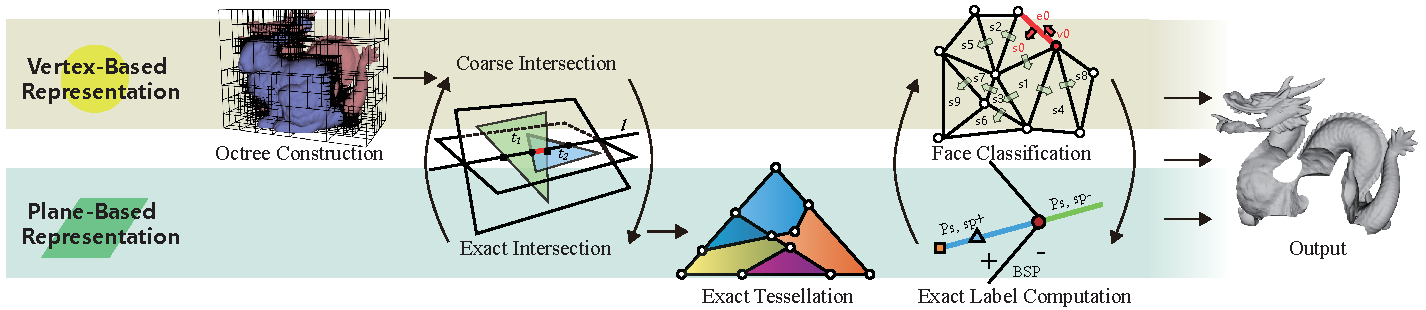
\includegraphics[width=7in]{overview}
	\caption{The illustration of our framework for boolean evaluation using hybrid representations. Vertex-based computation has its advantage of efficiency, and plane-based is necessary to guarantee exact geometry predicates. }\label{fig:hybrid}
\end{figure*}

\IEEEraisesectionheading{\section{Introduction}\label{sec:introduction}}
\IEEEPARstart{C}{onstructive} solid geometry (CSG) has long been a popular modeling tool for computer-aided design (CAD) and computer-aided manufacturing (CAM). Complex models are constructed by combining primitives using regularized boolean operations \cite{requicha1977mathematical,tilove1980closure}, namely, union, intersection, and difference. A CSG can be converted into the boundary representation (B-rep) through boolean evaluation. There are two major types of boolean evaluation methods, which vary according to how they deal with intersections between primitives.
Approximate methods \cite{wang2011approximate,pavic2010hybrid,biermann2001approximate} rediscretize \hongbo{why re-?} intersection areas, fit vertices approximatively, and rearrange the topology.
In constrast, exact methods \cite{ogayar2015deferred,douze2015quickcsg,zhou2016mesh} do not change vertex positions, and maintain as many input elements (such as faces, vertices, and topology) as possible. In many applications, exact methods are preferred for their accuracy. Additionally, the clear mapping between the surfaces of the input and output meshes in exact methods simplifies the inheritance of surface information, such as face colors and materials.



However, there is always a compromise between robustness and efficiency for exact boolean algorithms.
Robust methods often require exact arithmetic \cite{barki2015exact,zhou2016mesh}, which is significantly slower than normal floating-point arithmetic to evaluate.
Other methods only guarantee \textbf{quasi-robust} \hongbo{why boldface?} \cite{shewchuk1999lecture} by using unreliable techniques, such as epsilon-tweaking \cite{laidlaw1986constructive,feito2013fast,segal1990using} and numerical perturbation \cite{douze2015quickcsg}.
Recently, robust plane-based methods have been developed \cite{bernstein2009fast,campen2010exact} based on binary space partition (BSP) merging algorithms \cite{naylor1990merging,thibault1987set}.
The robustness of these methods is guaranteed by the theorem of Sugihara and Iri \cite{sugihara1990solid} that boolean evaluations can be performed without \textbf{constructions} \cite{shewchuk1999lecture} if polyhedrons are represented based on planes instead of vertices.
By using only \textbf{predicates}, it is easier to robust boolean methods.
These plane-based methods are generally faster than others which use exact arithmetic. However, they still suffer from performance issues because of the high computation complexity of BSP algorithms. In addition, the incoherence between BSP representations and B-reps of polyhedrons requires extra steps for conversion and connectivity reconstruction, leading to worse performance.


Inspired by these previous studies, we develop a robust boolean evaluation method, which is unconditionally robust given consistent solid inputs, and whose efficiency is comparable to non-robust methods. Our method combines P-reps with V-reps \hongbo{you should introduce P-rep and V-rep in the introduction again and make their advantages/disadvantages clear}, forming hybrid representations of solids, as illustrated in Figure~\ref{fig:hybrid}. Generally, the V-rep information is used for coarse tests and efficient neighboring face queries, while the P-rep information is used for exact predicates. To avoid using exact arithmetic and ensure efficiency, we avoid constructions throughout our method.
%
%\ca{making our method significantly faster than the previous BSP-based methods .}

%Our method is different from the previous BSP-based methods .
%While their methods are largely based on BSP theorem of \cite{naylor1990merging,thibault1987set}, our method is more like  and is . 

\ca{Our method is more like vertex-based methods such as \cite{feito2013fast,zhou2016mesh} \hongbo{you didn't introduce vertex-based methods before} than BSP-based methods \cite{bernstein2009fast,campen2010exact}. However, we provide a systematical solution for robust boolean evaluations, instead of a simple improvement of vertex-based methods}. \hongbo{what is the purpose of the following text? More about the methodology itself or the difference from vertex-based approaches?} During intersection computation, we encode triangle intersections into sets of planes, and then use these planes to determine exact tessellations. \hongbo{Are the discussions here related to Fig. 1? If yes, please refer to different parts of the figure here} Subsequently, we classify each face in the tessellated meshes using small local BSP trees, which also compliment the P-reps to guarantee exactness. In order to achieve fast performance, we minimize the usage of plane-based exact predicates in these stages. In addition, while most existing boolean methods can only process two meshes in each time, our method is \textbf{variadic} \cite{zhou2016mesh} \hongbo{you haven't explained the N-Mesh appeared in the title}, and thus can evaluate boolean expression with multiple input meshes immediately \hongbo{simultaneously?}, reducing the evaluation time of large CSGs by avoiding repetitive computation. Experiments have shown that our method is much faster than the existing robust methods \hongbo{REF}, and only around two times slower than non-robust methods \hongbo{REF}.

\section{Related Work}
\hongbo{Since the main contribution is about the hybrid representation, you'd better clearly and explicitly introduce the vertex-based and plane-based methods. In addition, if we have any contribution using ``N-Mesh'' boolean evaluation, you'd also discuss the relevant existing works as well.}

Boolean methods have been researched since their inception in the 1980s \cite{requicha1985boolean, laidlaw1986constructive}. Existing methods can be mainly divided into two categories: exact methods and approximate methods. Exact methods retain vertex positions, and the topology of the inputs is preserved as much as possible. The coordinates of intersection points between input meshes are computed by input configurations. However, the coordinates cannot be represented exactly using fixed-precision floating point numbers. Hence exact arithmetic is needed for robustness. In contrast, approximate methods rediscretize the input mesh surfaces using techniques like voxels, octrees, and Layered Depth Images (LDI). These methods generally have better performance and are often more robust than exact methods, but at the cost of relatively low precision and losing geometry information. 
\hongbo{It's expected you will comment whether the proposed technique is an exact or approximate method.}
In this section, we first introduce previous works of these two categories, and then discuss plane-based boolean methods, which have a close relation with our method.

\textbf{Exact Methods.}
Some exact methods (e.g., \cite{ogayar2015deferred,douze2015quickcsg,xu2013fast,feito2013fast,updegrove2016boolean}) are optimized for efficiency, but cannot guarantee robustness. Since they are implemented by fixed-precision floating-point arithmetic, numerical errors are inevitable and often lead to inconsistent results.
Douze et al. \cite{douze2015quickcsg} developed a very efficient method for handling very large meshes and arbitrary input primitives. However, their method makes a general position assumption and cannot deal with coplanar situations\hongbo{it's not clear why a general position assumption doesn't allow coplanar cases. in addition, you'd better comment if your method can handle coplanar cases}.

Some other methods focus more on achieving robustness. For example, the state-of-art method \cite{zhou2016mesh} tries to handle a large range of topology deficiencies and guarantees solid outputs, with the cost of many extra computations such as self-intersecting tests and vertex-rounding iterations.
Since the robustness problem is often due to numerical errors, many researchers have attempted use arbitrary precision arithmetic \cite{banerjee1996topologically, fortune1995polyhedral, keyser2004esolid, granados2003boolean, hachenberger2005boolean, zhou2016mesh,barki2015exact} and exact interval computation \cite{fang1993robustness, hu1996robust, segal1990using}. However, exact arithmetic is computationally very expensive. For example, CGAL's \cite{cgal:hk-bonp3-15a} exact-arithmetic implementation \cite{granados2003boolean} of Nef polyhedra \cite{bieri1988elementary} is more than 50 times slower than non-robust boolean operations \cite{bernstein2009fast} \hongbo{why cite this work here? It is a robust plane-based approach?}. We aim to balance the performance and robustness, which guarantees solid outputs under valid inputs but without the use of exact arithmetic.


\textbf{Approximative Methods.}
Since it is difficult to achieve efficiency, accuracy, and robustness at the same time, some methods \hongbo{REF} sacrifice accuracy for greater efficiency and robustness. Most of such methods are based on volumetric representations of meshes. However, the quality of their results highly depends on the resolution of the volume grids, and better quality requires significantly higher resolutions.
To accelerate this process, some methods reduce the complexity of output meshes \cite{varadhan2004topology}, whereas others preserve non-intersected areas of input meshes to avoid redundant tessellation \cite{pavic2010hybrid,wang2011approximate,zhao2011parallel,hable2005blister,ogayar2006gpu,updegrove2016boolean}.
Moreover, with the development of general-purpose computing on graphics processing units (GPGPU), many of them utilize the computational power of graphics hardware for accelerating boolean evaluations. These methods achieve good performance, and thus are suitable for interactive applications. However, the fundamental problem of approximate methods arises from the grid-dependent nature of volumetric calculations. They inevitably suffer from geometric detail loss and unwieldy topological changes.
\hongbo{one sentence about our method}

\textbf{Plane-Based Methods.}
\label{sec:pbrelated}
The concept of plane-based representations (P-reps) of polyhedrons was first introduced by Sugihara and Iri \cite{sugihara1990solid}. By using the P-reps, boolean evaluations can be performed with only predicates, which are much easier to implement robustly \hongbo{than what?}. Berstein and Fussell \cite{bernstein2009fast} combined the P-reps with BSP trees \cite{thibault1987set,naylor1990merging} to develop a boolean evaluation method which is unconditionally robust with consistent inputs. Unlike vertex-based methods \hongbo{REF; again, no previous discussion on vertex-based methods yet}, their method \ca{is robust but without relying on exact arithmetic\hongbo{correct?}}
However, the merging of two BSP trees has $O(mn)$ time complexity, where $m$ and $n$ are the sizes of the trees. Such high time complexity\hongbo{only $O(m^2)$, not that computationally expensive?} makes this method impractical for large meshes. Subsequently, Campen and Kobbelt \cite{campen2010exact} improved this method by localizing BSP operations using an octree. In their method, mesh refinements only take place locally near intersections, leading to better performance. However, their method splits the intersection regions and non-intersection regions, and requires an extra stitching step to reconstruct topology. Also, the performance of localized BSP merging is still poor compared with the vertex-based methods. Our method uses plane-based geometry to guarantee no error introduced during boolean evaluation, while reducing the performance cost for plane-based computation with the V-rep information, which is much cheaper to use.
